\begin{figure}[H]
	\centering
	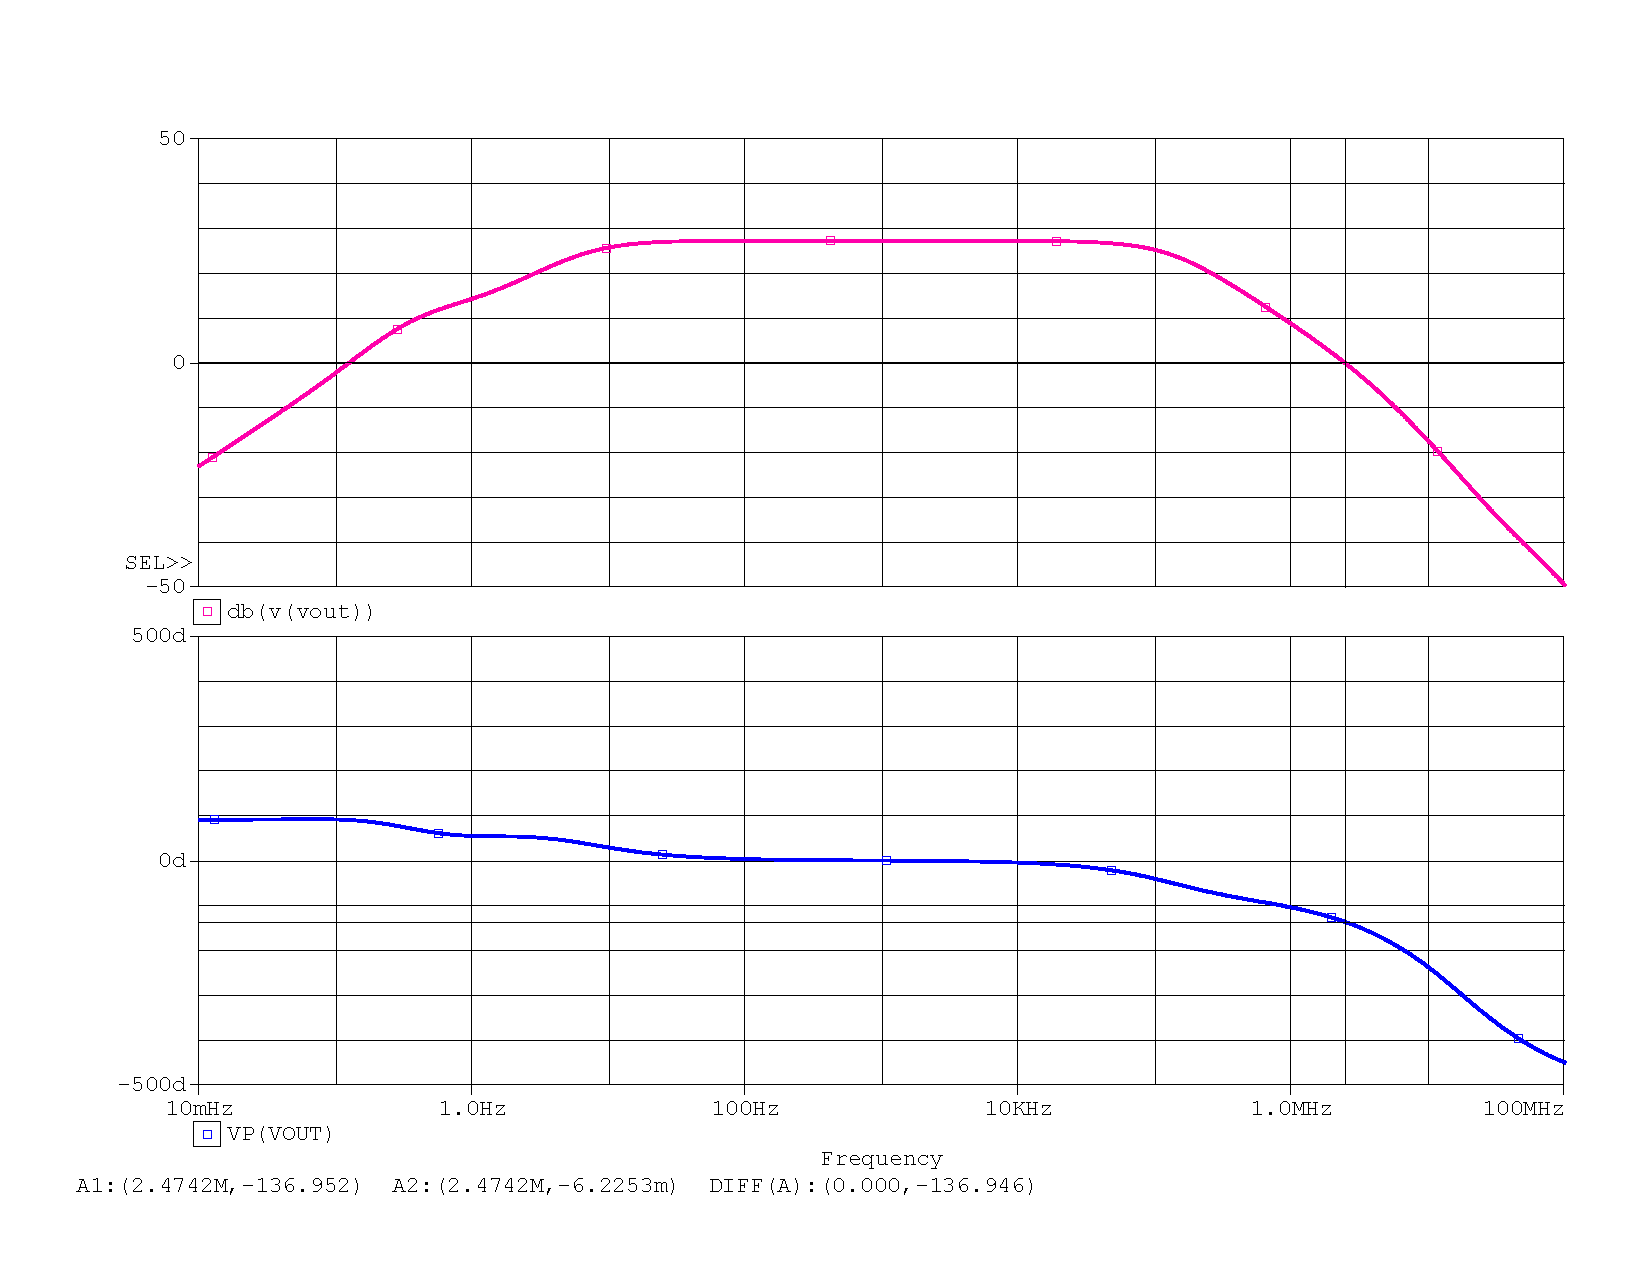
\includegraphics[scale=0.4]{sim_bode_400p.pdf}
	\caption{Diagrama de Bode.}
	\label{fig:sim_bode}
\end{figure}

En la Figura \ref{fig:sim_bode} se presentan la magnitud y fase en la salida en función de la frecuencia.
El margen de fase se define como el ángulo que le falta a \SI{-180}{\degree} para llegar a la fase cuando la ganancia es \SI{0}{\decibel}. Para determinar su valor, se busca en la Figura \ref{fig:sim_bode} el punto de cruce de la gráfica de magnitud con \SI{0}{\decibel}, que corresponde a una frecuencia de \SI{2.5}{\mega\hertz}. La fase en dicha frecuencia es de \SI{-136}{\degree}, por lo que el margen de fase resulta:

	$$ \mathrm{MF} = \SI{-180}{\degree} + \SI{136}{\degree} = \boxed{\SI{-44}{\degree}} $$